\subsection{Загрузка и запуск программы}
Приложение доступно по веб-адресу \url{http://gcsales.ru}\\
Для начала работы достаточно просто перейти по данному адресу, установка
программы не требуется.

\subsection{Использование приложения}
При успешном запуске, пользователь должен увидеть следующий интерфейс:
\begin{figure}[H]
    \centering
    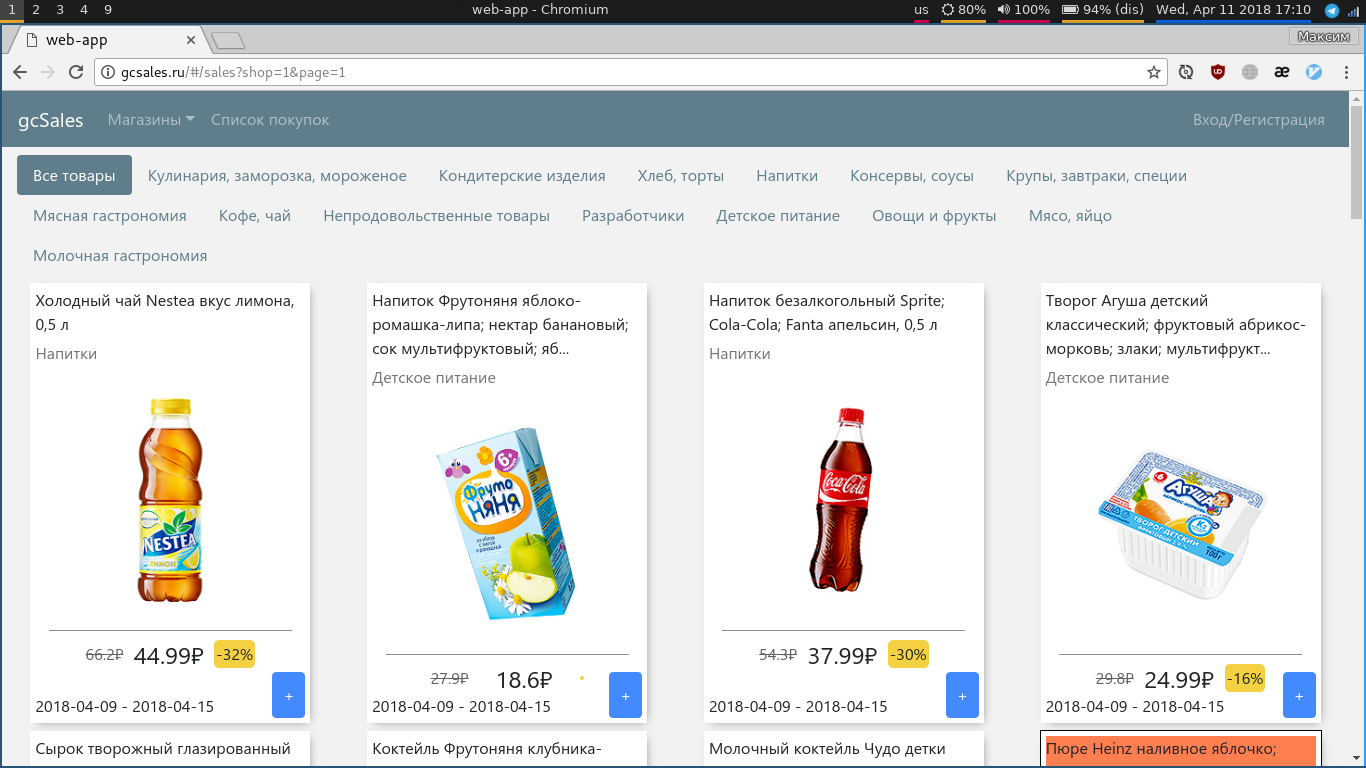
\includegraphics[width=\textwidth]{./screenshots/interface_main.png}
    \caption{Главная страница приложения}
\end{figure}
На этом экране можно выбрать магазин, акции которого нужно отобразить, по
умолчанию товары отображаются общим списком, для того, чтобы выбрать товары
определенной категории, нужно нажать на одну из кнопок, например <<Кофе, чай>>.
Пользователь может добавить товар в список покупок, нажав на кнопку <<+>> в
карточке товара.

Для того, чтобы начать пользоваться списком покупок, пользователю необходимо
авторизоваться в системе. После чего нужно нажать на ссылку <<Список покупок>>
в меню навигации.
\begin{figure}[H]
    \centering
    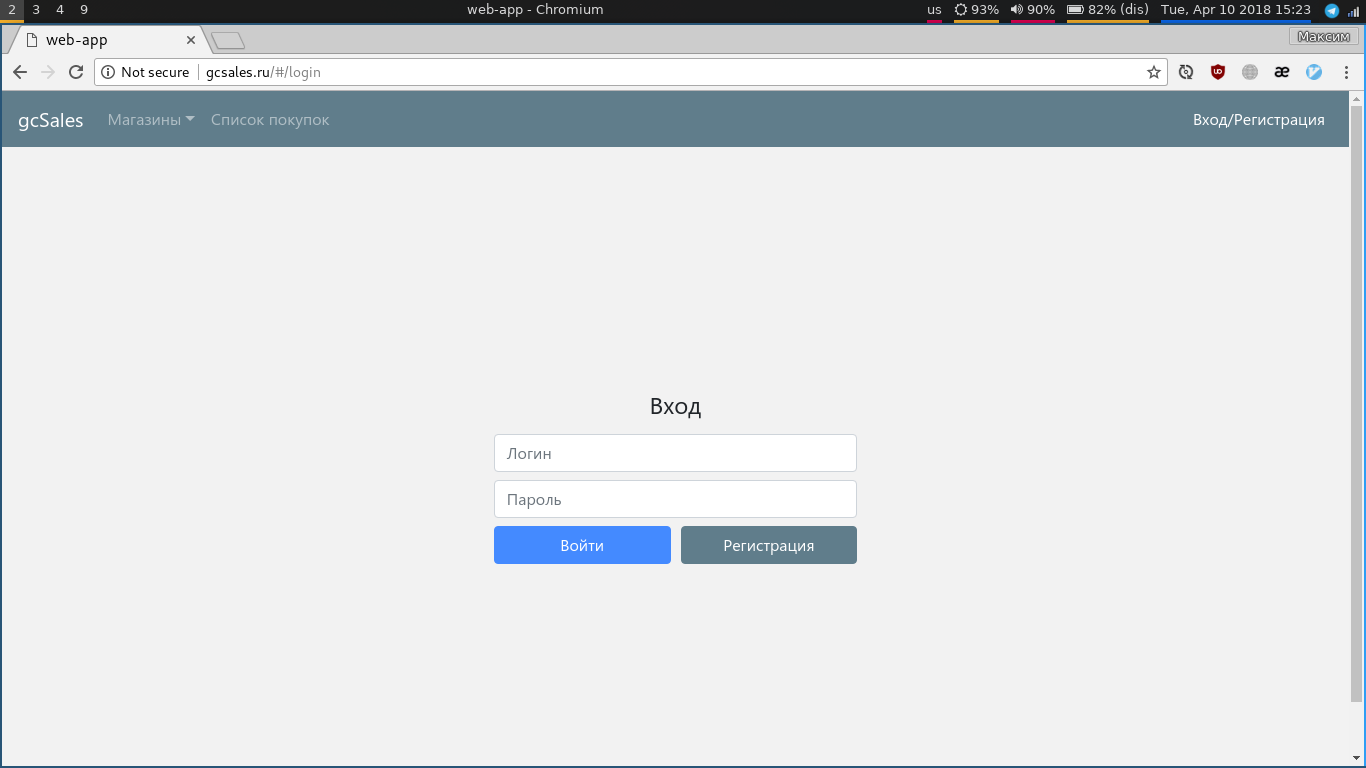
\includegraphics[width=\textwidth]{./screenshots/login.png}
    \caption{Авторизация в системе}
\end{figure}

Для начала нужно создать список покупок (у пользователя может быть несколько
списков покупок). Для этого нужно нажать кнопку <<Добавить>>.
\begin{figure}[H]
    \centering
    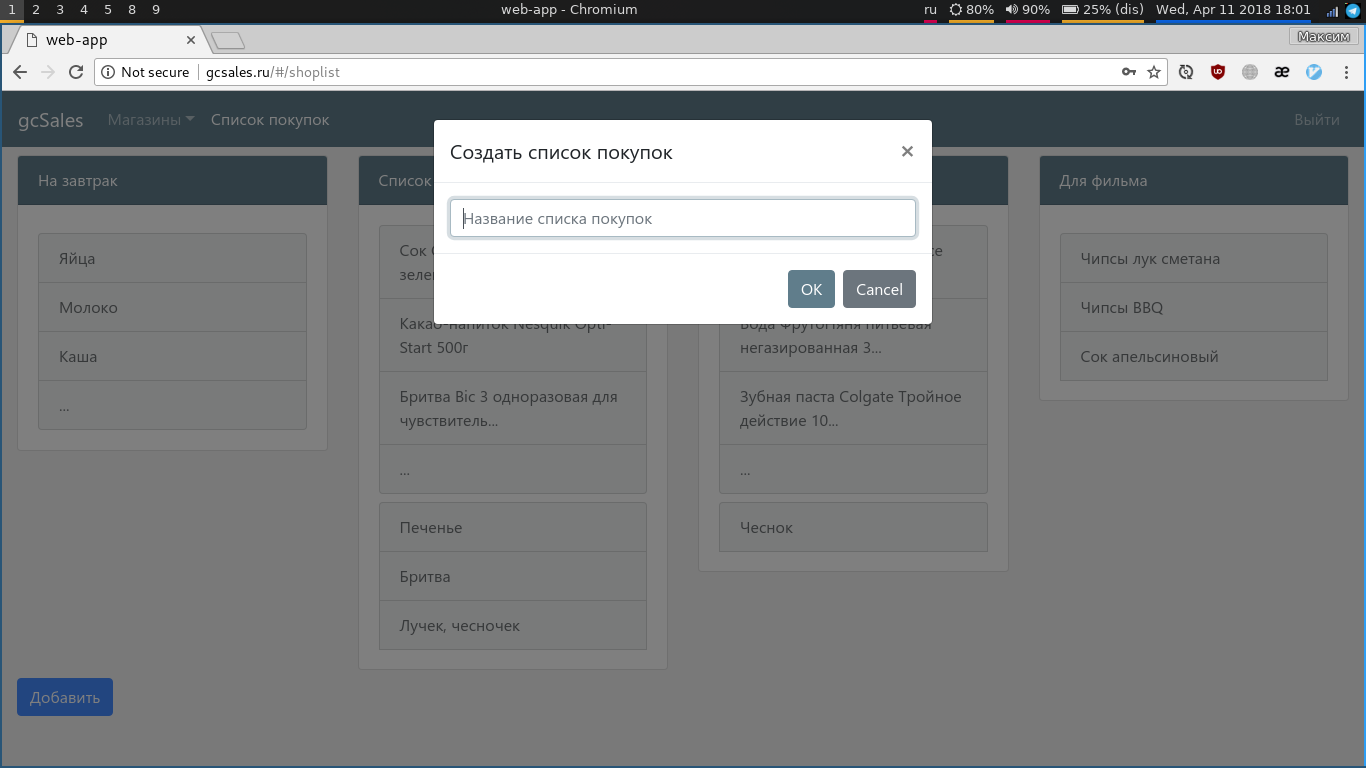
\includegraphics[width=\textwidth]{./screenshots/create_shoplist.png}
    \caption{Создать список покупок}
\end{figure}

Список покупок выглядит следующим образом: 
\begin{itemize}
  \item Слева находятся товары магазинов, которые пользовать добавлял, нажимая
    на кнопку <<+>> в карточке товара.
  \item Справа находятся пользовательские позиции, которые можно добавлять,
    вводя их название в текстовое поле. Для пользовательской позиции можно
    посмотреть рекомендации (при нажатии на название раскрывается список).
  \item Внизу находится общая сумма покупок и кнопка удаления списка покупок.
\end{itemize}

Пользователь также может удалять товары из списка покупок, нажимая кнопку <<->>
в карточке товара. Также можно удалить и сам список покупок, нажав на кнопку
<<Удалить список покупок>> внизу экрана.

\begin{figure}[H]
    \centering
    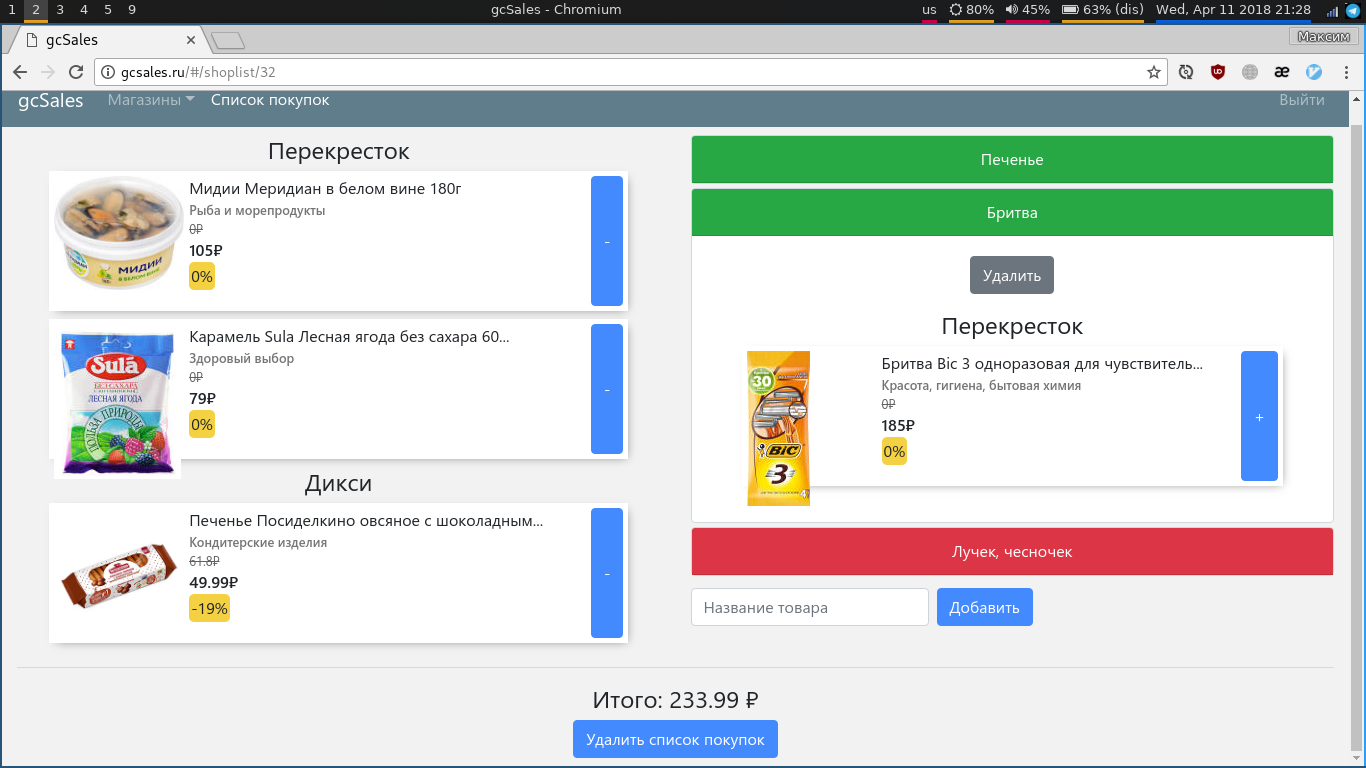
\includegraphics[width=\textwidth]{./screenshots/shoplist.png}
    \caption{Список покупок}
\end{figure}

